\documentclass[12pt]{article}
\usepackage{fancyhdr,nameref}
\usepackage[a4paper,margin=1cm,top=1in,footskip=0.5cm]{geometry}
\usepackage{enumitem}
\usepackage{listings}
\usepackage{courier,caption,soul}
\usepackage{amsmath,amsfonts,fixmath}
\usepackage{tabu,array,graphicx}
\usepackage[nodayofweek]{datetime}
\usepackage[usenames,dvipsnames]{xcolor}
\usepackage{pgfplots}
\usepackage{circuitikz,siunitx}
\usepackage{titlesec}
\usepackage{tabto}
\usepackage[absolute]{textpos}
\usepackage{pdflscape}
\usepackage{pdfpages}
\usepackage{makecell}
\usepackage{multirow}
\pgfplotsset{compat=1.12}
\everymath{\displaystyle}
\setlength\extrarowheight{4pt}
\newdateformat{datef}{\twodigit{\THEDAY}{ }\shortmonthname[\THEMONTH]{ }\THEYEAR}
\newdate{date}{17}{07}{2015} % parameters are DDMMMYYYY format; output is DD MMM YYYY format
\pagestyle{fancy}
\fancyhf{}
\fancyhf[FC]{\thepage}
\fancyhf[HL]{\slshape COSC 2203-01}
\fancyhf[HC]{\scshape Component A}
\fancyhf[HR]{\slshape \leftmark}
\newcommand{\hlc}[2][yellow]{ {\sethlcolor{#1} \hl{#2}} }
\newcommand{\hlbox}[1]{\colorbox{cyan!50}{#1}}
\newcommand{\qw}[1]{\si{.#1}}
%\titleformat*{\section}{\LARGE\bfseries\ttfamily}
\definecolor{dkgreen}{RGB}{0,102,0}
\definecolor{gray}{rgb}{0.5,0.5,0.5}
\definecolor{mauve}{rgb}{0.58,0,0.82}
\lstset{frame=tb,
	escapeinside={\%*}{*)},
	captionpos=t,
	language=Java,
	aboveskip=3mm,
	belowskip=3mm,
	showstringspaces=false,
	columns=flexible,
	basicstyle={\small\ttfamily},
	numbers=none,
	numbersep=0pt,
	numberstyle=\small\ttfamily\color{gray},
	keywordstyle=\color{blue},
	commentstyle=\color{dkgreen},
	stringstyle=\color{mauve},
	breaklines=true,
	breakatwhitespace=true,
	tabsize=3}
\begin{document}
\newcolumntype{C}{>{\centering\arraybackslash}p{1em}}
	
	\begin{titlepage}
\newcommand{\HRule}{\rule{\linewidth}{0.5mm}} % Defines a new command for the horizontal lines, change thickness here

\center % Center everything on the page
 
%----------------------------------------------------------------------------------------
%	HEADING SECTIONS
%----------------------------------------------------------------------------------------

\textsc{\LARGE LeTourneau University}\\[1.0cm] % Name of your university/college
\textsc{\Large COSC 2203-01}\\[0.5cm] % Major heading such as course name
\textsc{\large Data Structures}\\[0.5cm] % Minor heading such as course title

%----------------------------------------------------------------------------------------
%	TITLE SECTION
%----------------------------------------------------------------------------------------

\HRule \\[0.4cm]
{ \huge \bfseries Programming Assignment \#3\\Component A}\\[0.2cm] % Title of your document
\HRule \\[1.5cm]
 
%----------------------------------------------------------------------------------------
%	Problem Set Section
%----------------------------------------------------------------------------------------

{\Large\bfseries ``Huffman Encoding''}\\[5mm]
{\Large \emph{Using Heaps and Binary Trees}} \\[1.5cm]


%----------------------------------------------------------------------------------------
%	AUTHOR SECTION
%----------------------------------------------------------------------------------------
\begin{minipage}{0.35\textwidth}
	\begin{flushleft} \large
		\emph{Author:}\\
		Brian \textsc{Scott} % Your name
	\end{flushleft}
\end{minipage}
~
\begin{minipage}{0.35\textwidth}
	\begin{flushright} \large
		\emph{Presented to:} \\
		Dr. Brent \textsc{Baas} % Supervisor's Name
	\end{flushright}
\end{minipage}\\[4cm]

%----------------------------------------------------------------------------------------
%	DATE SECTION
%----------------------------------------------------------------------------------------

{\large \datef\displaydate{date}}\\[2cm] % Date, change the \today to a set date if you want to be precise

%----------------------------------------------------------------------------------------
%	LOGO SECTION
%----------------------------------------------------------------------------------------
\vfill % Fill the rest of the page with whitespace

\includegraphics[scale=0.20]{logoHoriz.jpg}\\[1cm] % Include a department/university logo - this will require the graphicx package
 
%----------------------------------------------------------------------------------------

\end{titlepage}
	\section{Problem Description}
	This program takes a set of strings and places them in a binary tree for the purpose of Huffman encoding. Huffman encoding of characters reduces the total space requirements by assigning short encodings to characters occurring more frequently, and longer encodings to those less frequent. We will use a binary tree to represent the Huffman encoding. The leaves of the tree are the characters being encoded. After encoding the strings, the program allows the user to decode a string based on the newly created Huffman tree.
	
	\section{Input / Output Analysis}
	\subsection{Input}
	Input constraints:
	\begin{itemize}
		\item Each string is $\leq$ 80 characters
		\item Each string contains no whitespace or punctuation
		\item Number of strings is $\leq$ 1,000,000
		\item Huffman-encoded string consists of zeros and ones
	\end{itemize}
	The program uses the regular expressions metacharacter \verb|\W| to remove whitespace and punctuation, and all characters are converted to lowercase. If only a blank line is entered, the program will terminate.
	\begin{lstlisting}[caption=Sample plaintext input]
		USA
		won
		the
		world
		cup
		and
		joe
		likes
		fat
		hotdogs
	\end{lstlisting}
	\vspace{1cm}
	\begin{lstlisting}[caption=Sample encoded input]
		101010011111101100010011011
	\end{lstlisting}
	\newpage
	
	\subsection{Output}
	
	\subsubsection{Example Output:}
	The output of the program is a table of each character, its frequency, and its Huffman code. The program then displays some statistics about the Huffman tree: its height, how many unique characters there are, and which characters had the longest and shortest encodings. When the user inputs a Huffman-encoded string, the program will display the plaintext of the encoded string. The program will prompt for encoded strings until the user types the word ``quit''.
	\begin{lstlisting}
	Enter some strings. Type a blank line when finished.
	USA 
	won 
	the
	world 
	cup 
	and 
	joe 
	likes 
	fat 
	hotdogs
	
	Input analysis complete.
	FREQ    CHAR    CODE
	-----------------------
	1       c       00000
	1       f       00001
	1       g       01001
	1       i       01110
	1       j       01111
	1       k       01000
	1       p       00110
	1       r       00111
	2       h       1010
	2       l       0001
	2       n       0101
	2       u       0010
	2       w       0110
	3       a       1100
	3       d       1101
	3       e       1110
	3       s       1011
	3       t       1111
	5       o       100
	Unique chars in tree: 19
	Tree Height: 5
	Longest Encoding: [00000 = c]
	Shortest Encoding: [100 = o]
	Enter a string to be decoded:
	101010011111101100010011011
	hotdogs
	Enter a string to be decoded:
	quit
	Program terminated
	\end{lstlisting}

	\newpage
	
	\section{Program Design}
	\subsection{Class Diagram}
	\begin{center}
		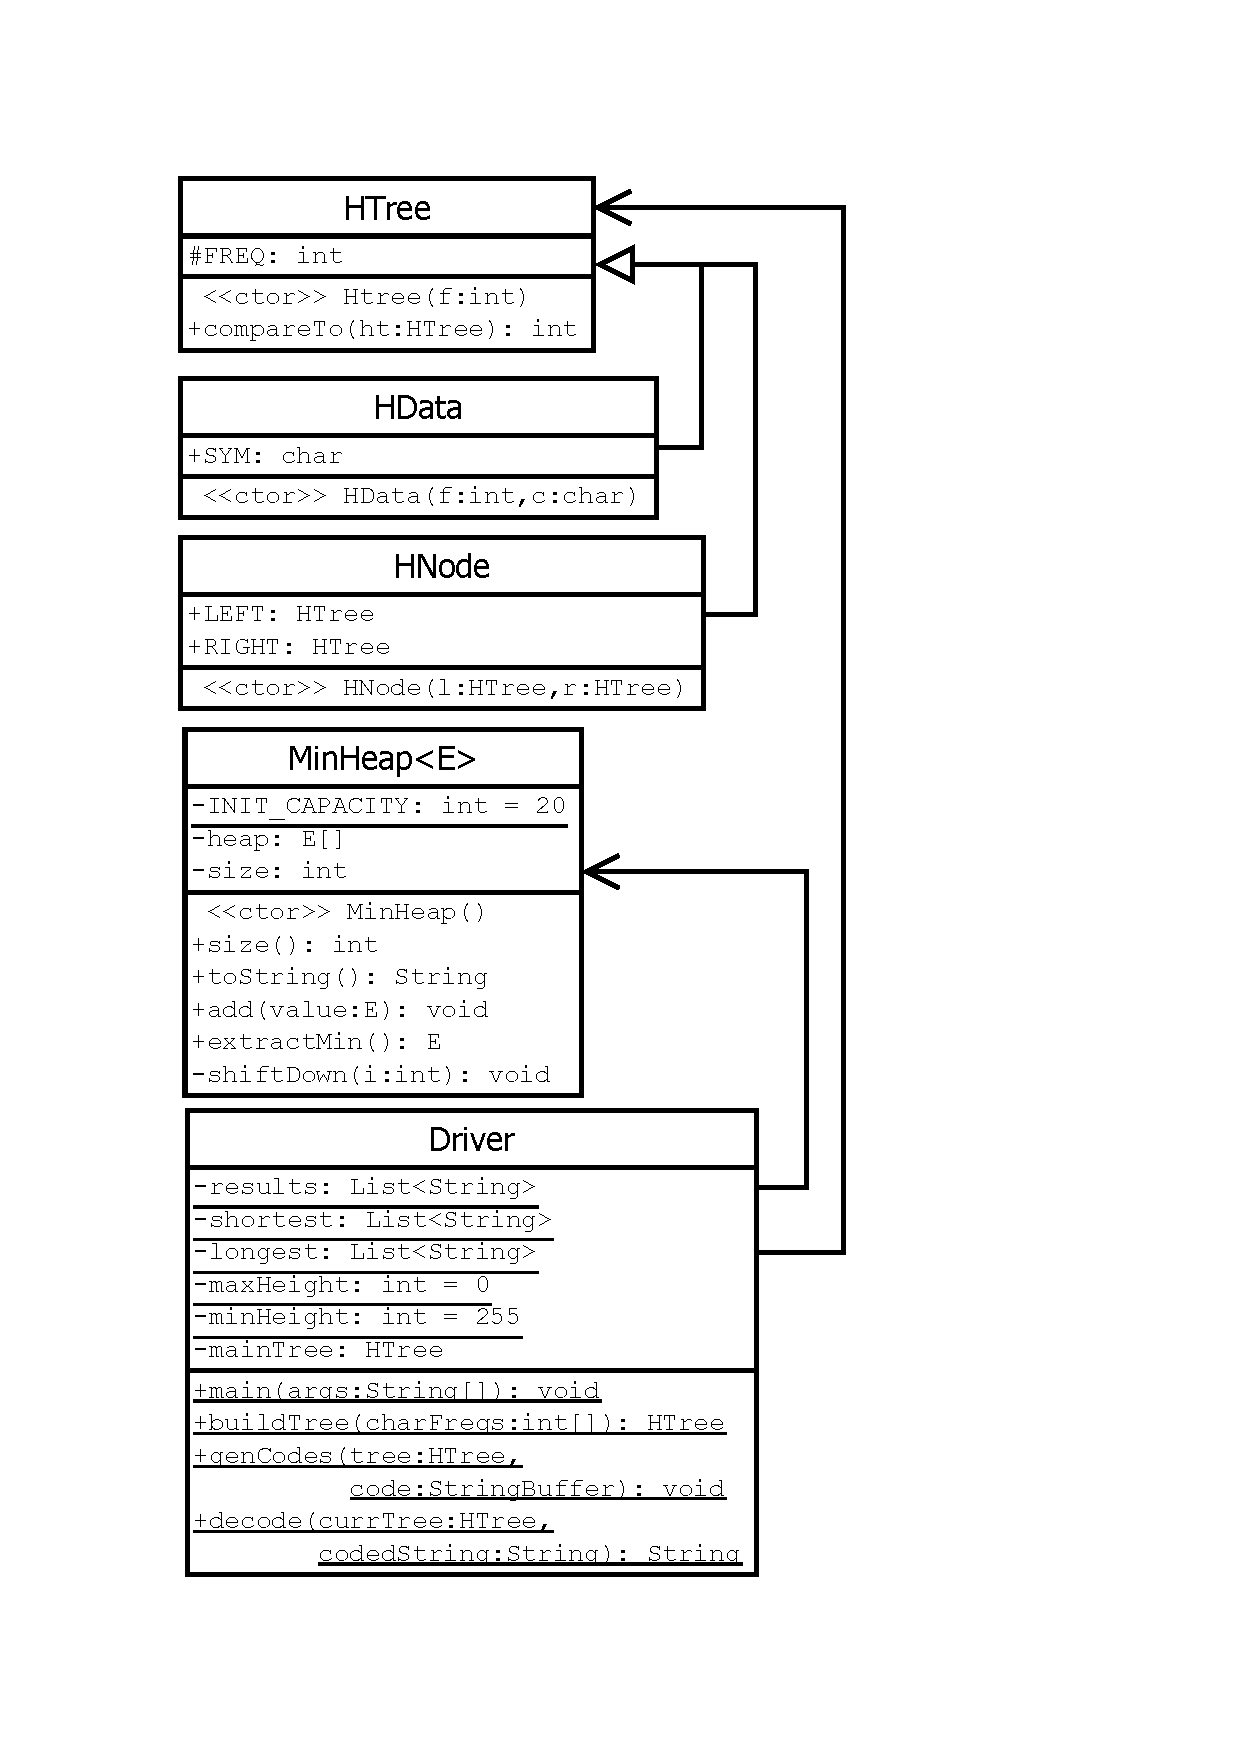
\includegraphics[scale=0.80]{3/cd.pdf}
	\end{center}
	\newpage
	\thispagestyle{empty}
	\begin{landscape}
		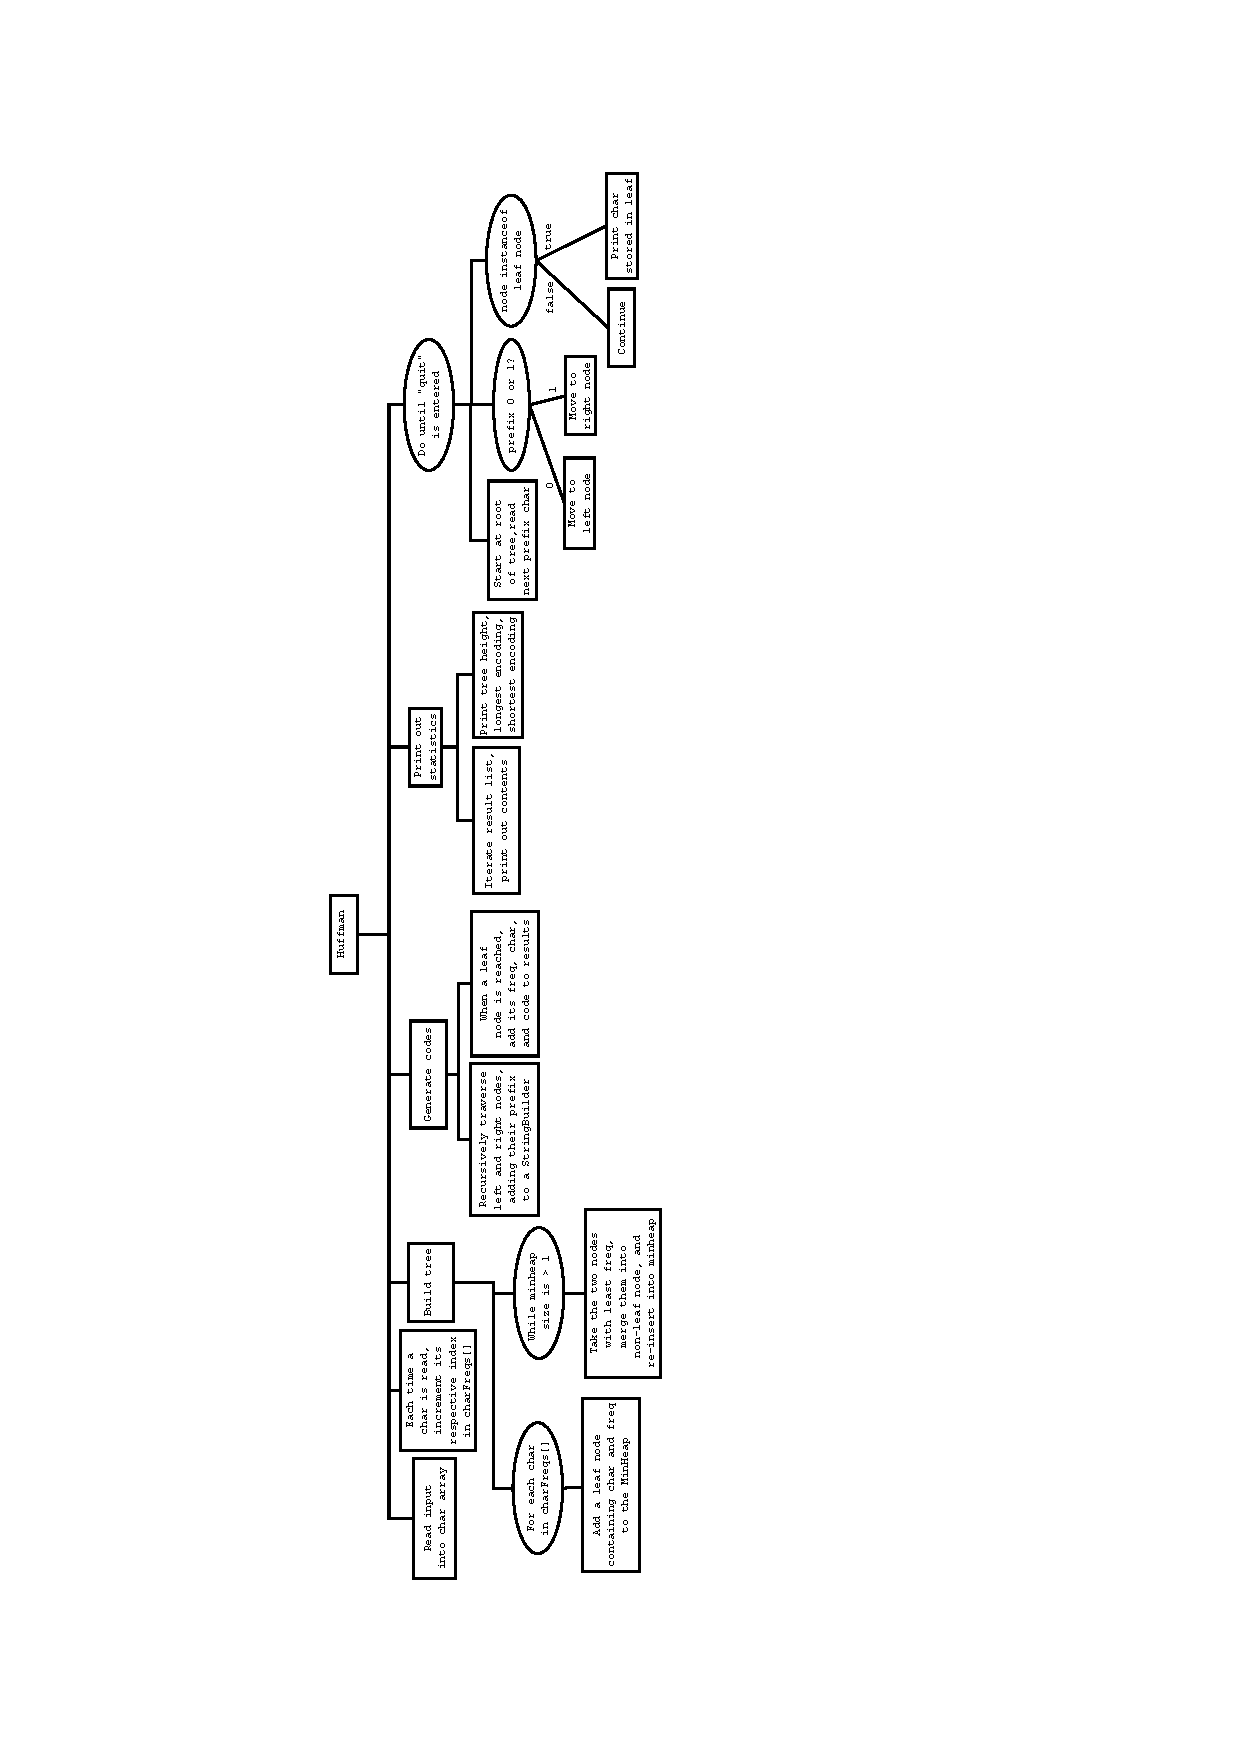
\includepdf[pages={1},scale=1.23,pagecommand=\subsection{Design Chart}]{3/deschart.pdf}
	\end{landscape}

	
	\section{Data Structure Graphics}
	\subsection{Min Heap:}
	\begin{center}
		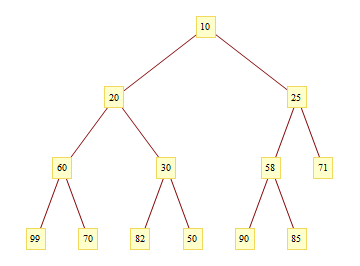
\includegraphics[scale=1.0]{min-heap.png}
	\end{center}
	\subsection{Huffman Tree:}
	\begin{center}
		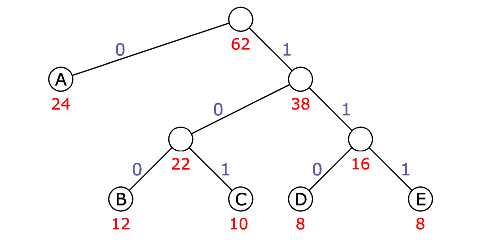
\includegraphics[scale=1.0]{hufftree.png}
	\end{center}

\end{document}